\section{Baseline}\label{sect:baseline}

The baseline algorithm defined in this study is a standard genetic algorithm (GA) that is used to optimize 
process allocation in cloud computing environments.
The GA is a stochastic population-based search algorithm that is based on the principles of natural selection and genetics.
It is a meta-heuristic that is used to find approximate solutions to optimization problems.

The GA is composed of the following components:
\begin{itemize}
    \item A population of candidate solutions;
    \item A fitness function that is used to evaluate the quality of each candidate solution;
    \item A selection operator that is used to select candidate solutions for reproduction;
    \item A crossover operator that is used to combine the selected candidate solutions to produce new candidate solutions;
    \item A mutation operator that is used to introduce random changes to the candidate solutions;
    \item A termination criterion that is used to determine when the GA should stop searching for solutions.
\end{itemize}

\begin{figure}[h]
    \centering
    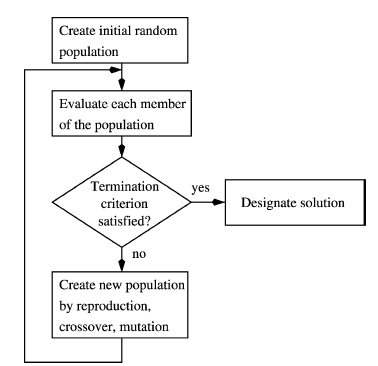
\includegraphics[width=0.5\textwidth]{./resources/examples/GAWorkflow.png}
    \caption{How a Genetic Algorithm works.}
    \label{fig:baseline}
\end{figure}
How a Genetic Algorithm (GA) works is shown in the flowchart~\cite{GAWorkflow} shown in Figure~\ref{fig:baseline}.

In this setting, the candidate solutions are represented by a list of tuples, each of which contains a Server and a list of Processes.
The initial population is generated by iterating over the Server list. For each Server, from the list of all the Processes, iteratively,
